%! Author = alida
%! Date = 18/12/2024

% Preamble
\documentclass[../main.tex]{subfiles}

% tutti i pacchetti usati vanno nel main

% Document
\begin{document}

    \section{Analisi}\label{sec:analisi}
%    \subfile{../../relazione/images}
        Nella fase di analisi, è stato effettuato un fit lineare ai dati
        appartenenti alla regione attiva delle caratteristiche in
        uscita, riportati nelle
        Tabelle~\ref{tab:100uA}~e~\ref{tab:200uA}.
        Per la precisione, al fine di ricavare i parametri
        desiderati direttamente dal fit, questo è stato eseguito
        secondo la funzione
        \begin{equation*}
            y = g \cdot ( x - V_A)
        \end{equation*}
        dove $g$ è la pendenza della retta, mentre $V_A$ rappresenta
        l'ascissa dell'intercetta con l'asse X.

        \begin{figure}[h!]
            \centering
            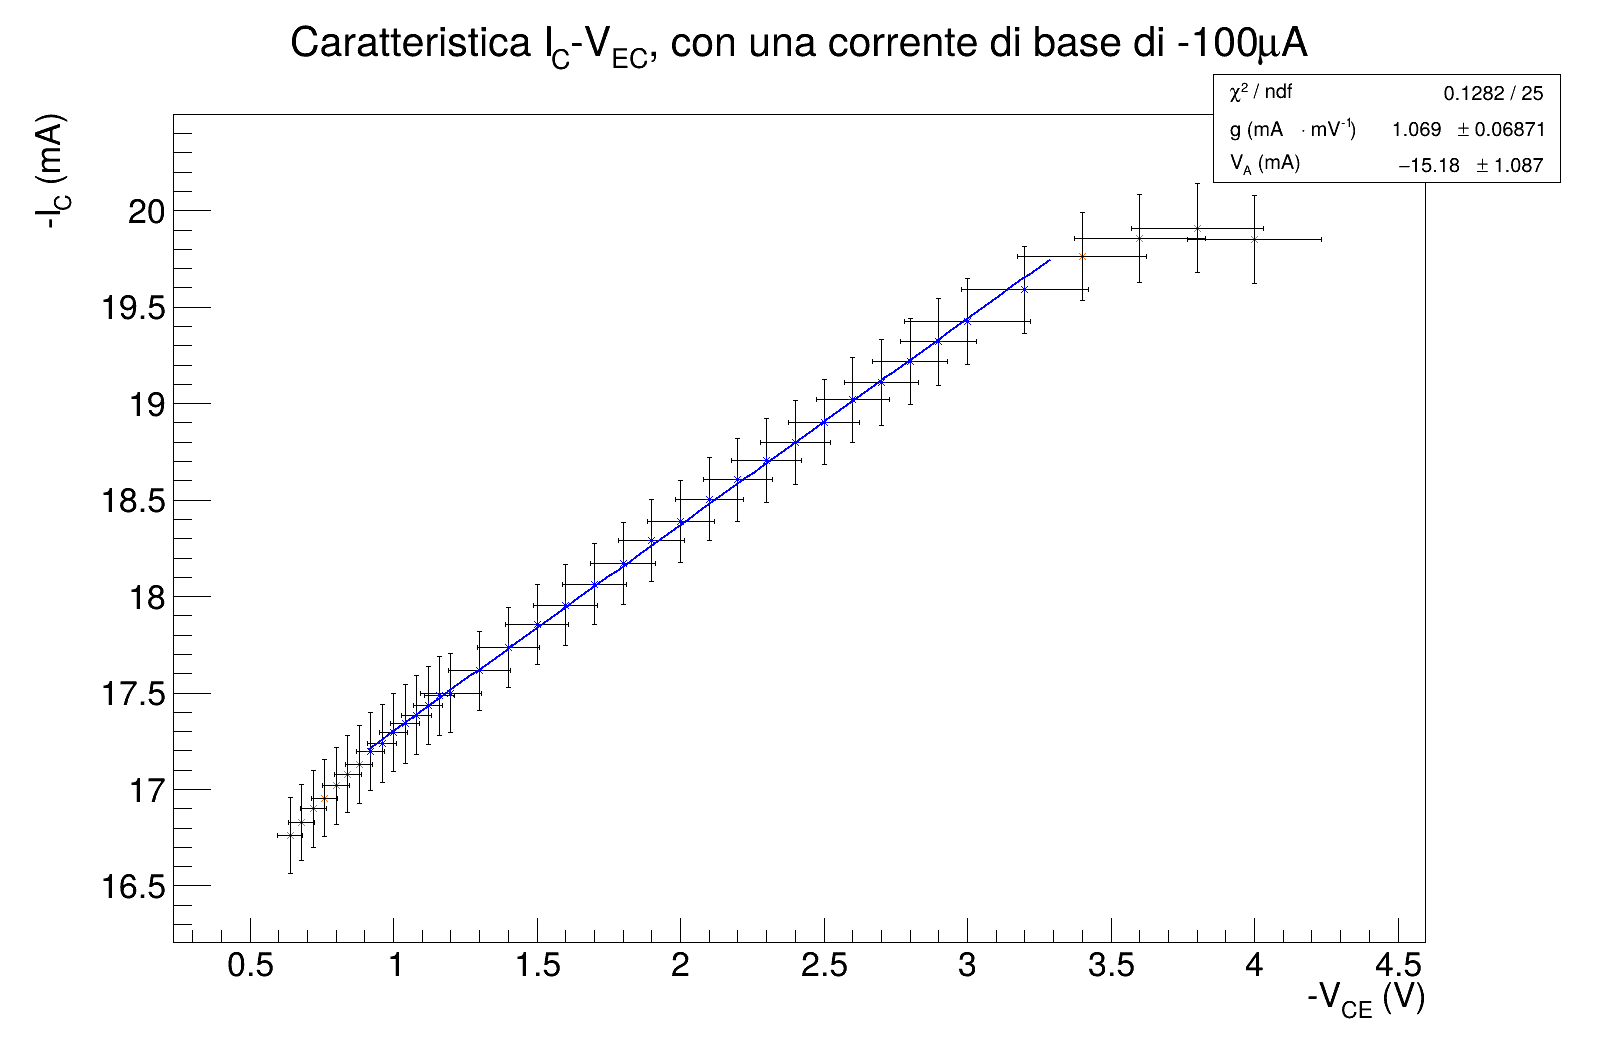
\includegraphics[width=.69\textwidth]{../../images/caratteristica-100uA}
            \caption{
                Grafico della caratteristica $I_C - V_{CE}$ ad assi
                invertiti e fit della regione attiva, con una
                corrente di base pari a 100 \textmu A.
            }
            \label{fig:fit-100}
        \end{figure}
        \begin{figure}[h!]
            \centering
            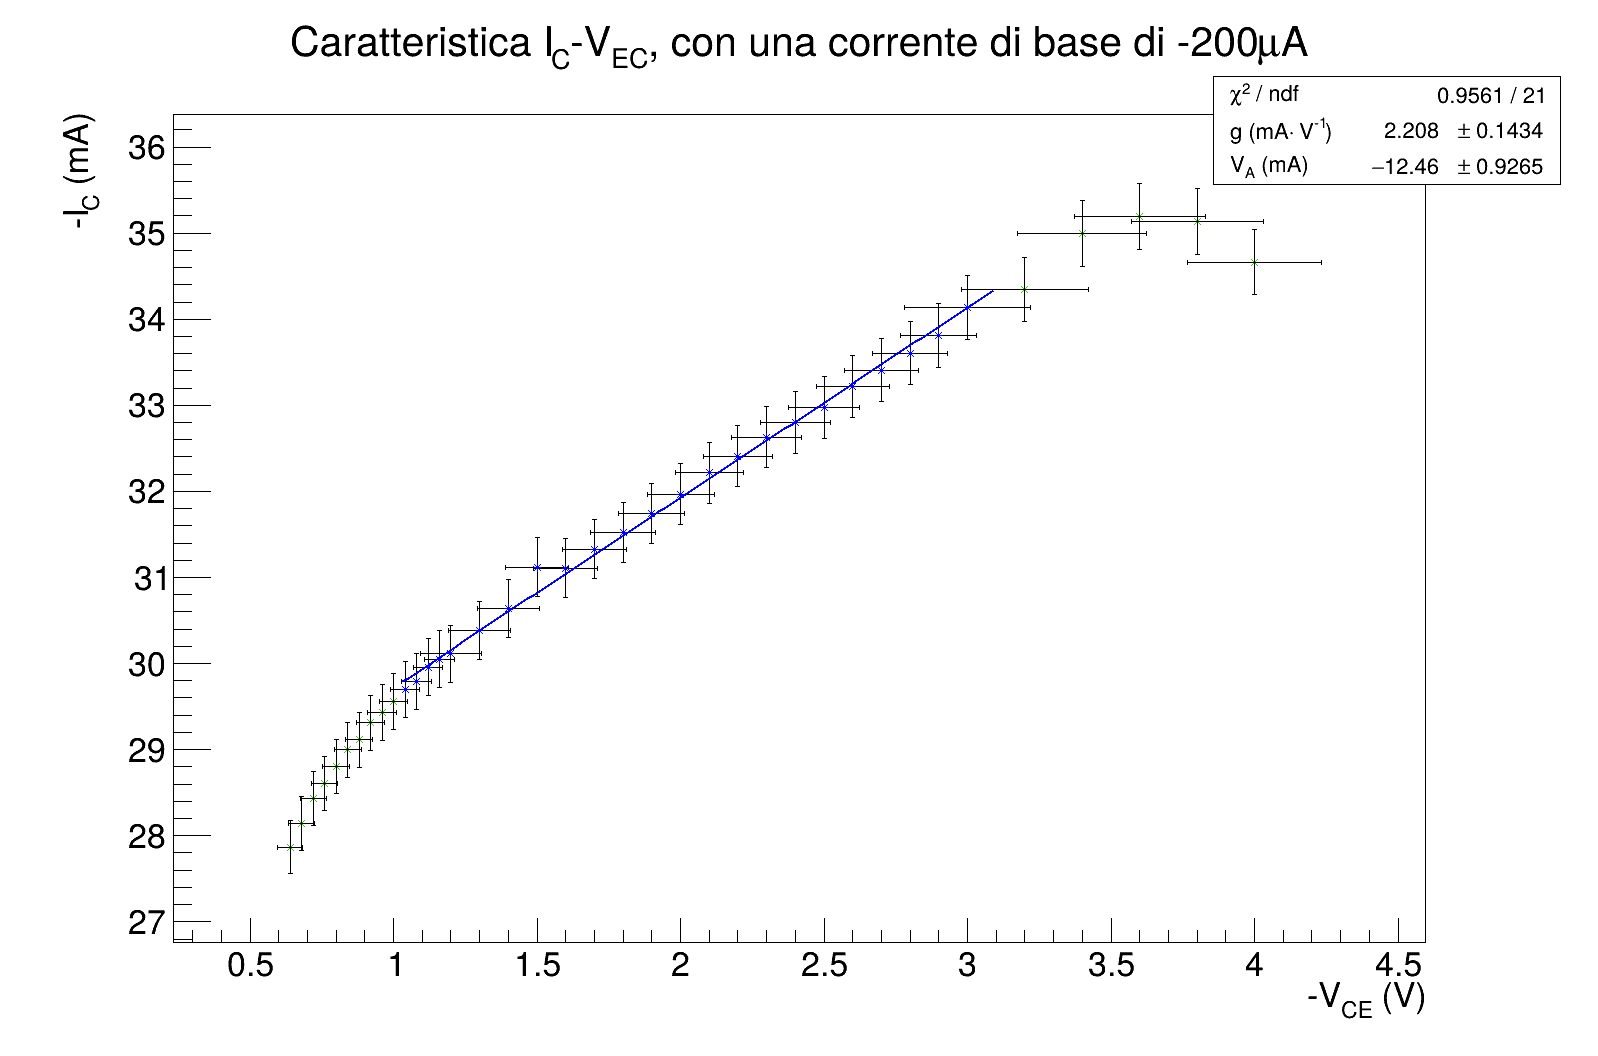
\includegraphics[width=.69\textwidth]{../../images/caratteristica-200uA}
            \caption{
                Grafico della caratteristica $I_C - V_{CE}$ ad assi
                invertiti e fit della regione attiva, con una
                corrente di base pari a 200 \textmu A.
            }
            \label{fig:fit-200}
        \end{figure}
        I risultati dei fit raffigurati nelle
        Figure~\ref{fig:fit-100}~e~\ref{fig:fit-200} sulle due
        caratteristiche sono rispettivamente:

    \begin{table}[ht]
        \centering
        \begin{subtable}[t]{.45\textwidth}
            \centering
            \begin{tabular}{||c|c||}
                \hline
                \multicolumn{2}{||c||}{Corrente di base di -100~\textmu A} \\
                \hline
                \rule{0pt}{3ex} $V_A$ (V) & $g$ (\textohm$^{-1}$) \\[1ex]
                \hline
                $15.2 \pm 1.1$    & $1.069 \pm 0.069$                                   \\
                \hline
            \end{tabular}
            \caption{-100}
            \label{tab:fit-100uA}
        \end{subtable}
        \hfill
        \begin{subtable}[t]{.45\textwidth}
            \centering
            \begin{tabular}{||c|c||}

                \hline
                \multicolumn{2}{||c||}{Corrente di base di -200~\textmu A} \\
                \hline

                \rule{0pt}{3ex} $V_A$ (V) & $g$ (\textohm$^{-1}$) \\ [1ex]
                \hline
                $12.46 \pm 0.93 $           & $2.21 \pm 0.14$                                          \\
                \hline
            \end{tabular}
            \caption{-200 \textmu A.}
            \label{tab:fit-200uA}
        \end{subtable}

        \vspace{0.5pt} % Spazio opzionale tra minipage e caption generale

        \caption{Risultati dei fit lineari effettuati sulle misure delle caratteristiche in uscita del transistor BJT,
            corrispondenti a una corrente di base di (a) -100\;\textmu A, (b) -200\;\textmu A.}
        \label{tab:fit_caratteristiche}

    \end{table}
    % TODO: capire quanle tabella ti piace di più
%    \begin{table}[ht]
%        \centering
%        \begin{tabular}{||c|c||}
%            \hline
%            \multicolumn{2}{||c||}{Corrente di base di -100\;\textmu A} \\
%            \hline
%            $V_A$ (\textnormal{A}) & $\varDelta V_{CE} / \varDelta I_C$ (\textohm) \\
%            \hline
%            $(...\pm...)\cdot $    & $...\pm...$                                   \\
%            \hline
%        \end{tabular}
%        \caption{Risultati dei fit lineari effettuati sulle misure delle caratteristiche in uscita del transistor BJT,
%            corrispondente a una corrente di base di -100\;\textmu A.}
%        \label{tab:fit-100uA}
%    \end{table}

%    \begin{table}[ht]
%        \centering
%        \begin{tabular}{||c|c||}
%            \hline
%            \multicolumn{2}{||c||}{Corrente di base di -200\;\textmu A} \\
%            \hline
%            $V_A$ (\textnormal{V}) & $\eta \varDelta V_{CE} / \varDelta I_C$ (\textohm)) \\
%            \hline
%            $(...\pm...)\cdot $    & $...\pm...$                                         \\
%            \hline
%        \end{tabular}
%        \caption{Risultati dei fit lineari effettuati sulle misure delle caratteristiche in uscita del transistor BJT,
%            corrispondente a una corrente di base di -200\;\textmu A.}
%        \label{tab:fit-200uA}
%    \end{table}

    I valori ottenuti dai fit sono stati utilizzati per calcolare
    il valore della resistenza in uscita $b$

    \begin{equation*}
        b = \frac{\varDelta V_{CE}}{\varDelta I_C} =
        \left( \frac{\varDelta I_C}{\varDelta V_{CE}} \right)^{-1} = g^{-1}
    \end{equation*}

    Si riportano tabulati in seguito i le stime dei valori di resistenza
    per correnti di base di -100~\textmu A e -200~\textmu A, calcolati mediante
    i valori riportati rispettivamente nelle
    Tabelle~\ref{tab:fit-100uA}~e~\ref{tab:fit-200uA}.

    \begin{table}[ht]
        \centering
        \begin{tabular}{||c|c||}
            \hline
            \multicolumn{2}{||c||}{Conduttanza di uscita} \\
            \hline
            $I_B$ (\textnormal{\textmu~A}) & $b$ (\textohm)) \\
            \hline
            $(-100\pm...) $                & $0.935 \pm 0.060$       \\
            \hline
            $(-200\pm...) $                & $0.453 \pm 0.029$       \\
            \hline
        \end{tabular}
        \caption{stima della conduttanza di uscita per due diversi valori di correnti di base, con incertezze.
        Per approfondire la valutazione delle incertezze si consulti Appendice ...} % TODO: mettere ref appendice
        \label{tab:resistenza}
    \end{table}

    In fine si è calcolato il guadagno di corrente $\beta(V_{CE})$ definito come:
    \begin{equation*}
        \beta(V_{CE}) = \frac{\varDelta I_C(V_{CE})}{\varDelta I_B} = \frac{\varDelta I_C(V_{CE})}{0.1}
    \end{equation*}

    \begin{figure}[h!]
        \centering
        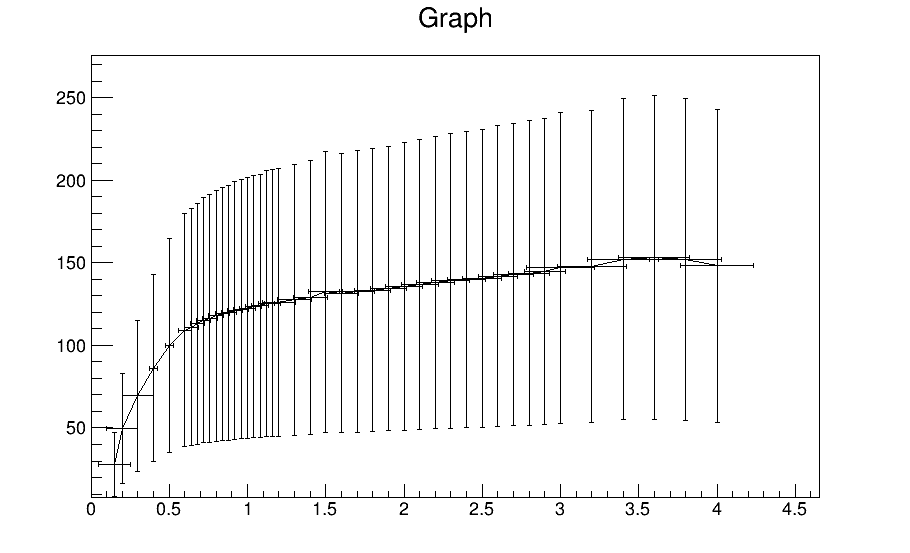
\includegraphics[width=0.7\textwidth]{../../images/beta}
        \caption{
            Grafico del guadagno di corrente $\beta$ in funzione di
            $V_{CE}$, tra i valori 100 e 200 \textmu A di $I_B$.
        }
        \label{fig:beta}
    \end{figure}
    È immediato notare l'entità degli errori sui valori di $\beta$
    riportati nel grafico in Figura~\ref{fig:beta}, per la
    spiegazione si veda l'appendice~... .
    Tar i punti nel grafico si riporta esplicitamente il valore $\beta(2) = 135 \pm  87$

%    Utilizzando i valori di conduttanza (Tabella~\ref{tab:conduttanza}) e le misure effettuate per le correnti di
%    base ... si vuole calcolare il guadagno di corrente,
%    \begin{equation*}
%        \centering
%        \beta (V_{CE}) = \frac{\varDelta I_C}{\varDelta I_B}
%    \end{equation*}
%
%    Al fine di garantire una stima più accurata, sono stati valutati i guadagni
%    per diversi valori di tensione $V_{CE}$ e successivamente ne è stata calcolata la media,
%    si riporta in seguito il risultato:
%
%    \begin{align*}
%        \centering
%        \beta = ... \pm ...
%    \end{align*}

\end{document}